% Created by tikzDevice version 0.12.3.1 on 2022-09-24 12:48:12
% !TEX encoding = UTF-8 Unicode
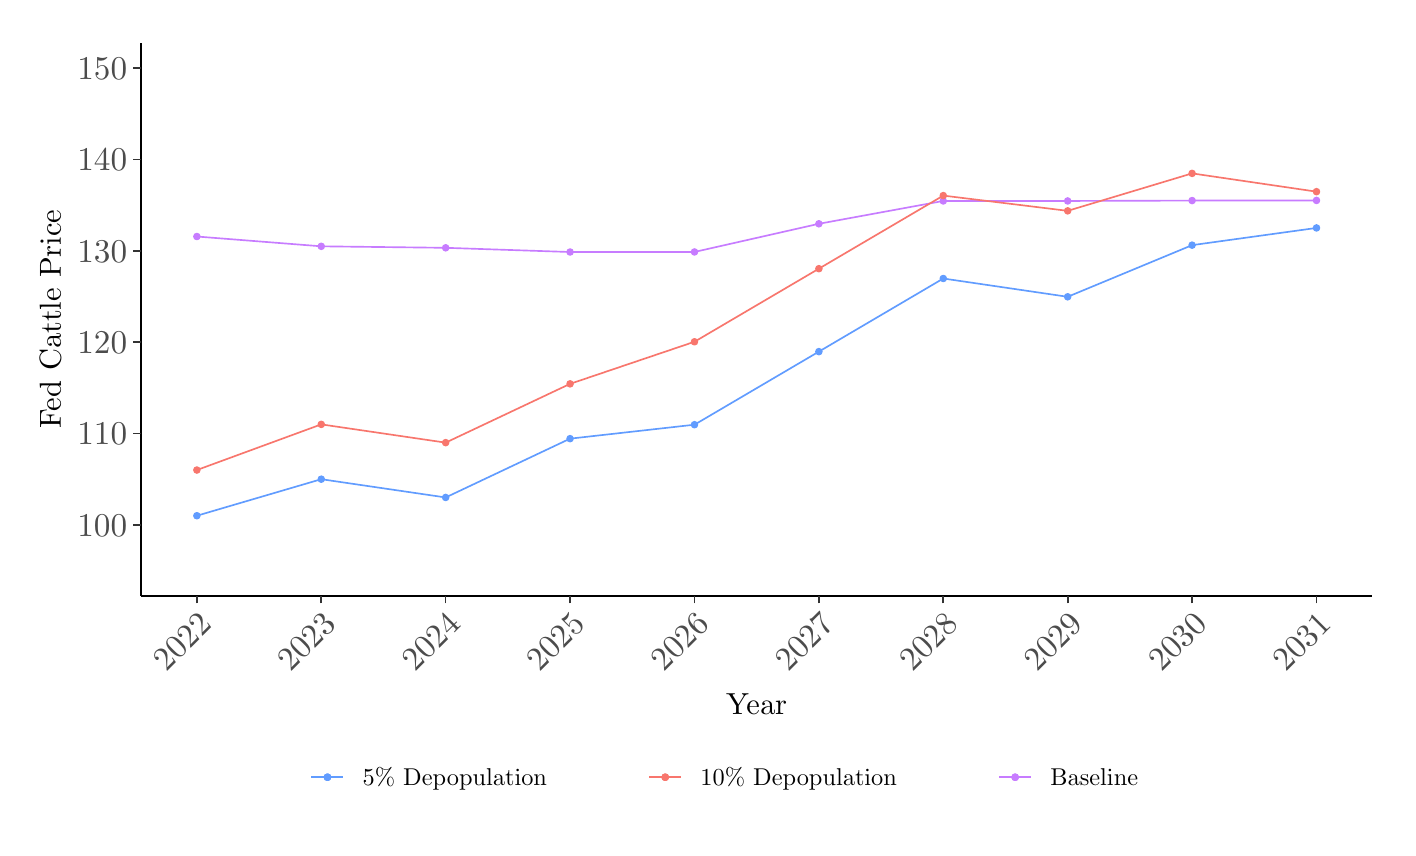
\begin{tikzpicture}[x=1pt,y=1pt]
\definecolor{fillColor}{RGB}{255,255,255}
\path[use as bounding box,fill=fillColor,fill opacity=0.00] (0,0) rectangle (491.44,289.08);
\begin{scope}
\path[clip] (  0.00,  0.00) rectangle (491.44,289.08);
\definecolor{drawColor}{RGB}{255,255,255}
\definecolor{fillColor}{RGB}{255,255,255}

\path[draw=drawColor,line width= 0.6pt,line join=round,line cap=round,fill=fillColor] (  0.00, -0.00) rectangle (491.44,289.08);
\end{scope}
\begin{scope}
\path[clip] ( 40.91, 83.83) rectangle (485.94,283.58);
\definecolor{fillColor}{RGB}{255,255,255}

\path[fill=fillColor] ( 40.91, 83.83) rectangle (485.94,283.58);
\definecolor{drawColor}{RGB}{199,124,255}

\path[draw=drawColor,line width= 0.6pt,line join=round] ( 61.14,213.61) --
	(106.09,210.07) --
	(151.04,209.53) --
	(195.99,208.01) --
	(240.95,208.03) --
	(285.90,218.21) --
	(330.85,226.46) --
	(375.80,226.46) --
	(420.76,226.60) --
	(465.71,226.65);
\definecolor{fillColor}{RGB}{199,124,255}

\path[draw=drawColor,line width= 0.4pt,line join=round,line cap=round,fill=fillColor] ( 61.14,213.61) circle (  1.16);

\path[draw=drawColor,line width= 0.4pt,line join=round,line cap=round,fill=fillColor] (106.09,210.07) circle (  1.16);

\path[draw=drawColor,line width= 0.4pt,line join=round,line cap=round,fill=fillColor] (151.04,209.53) circle (  1.16);

\path[draw=drawColor,line width= 0.4pt,line join=round,line cap=round,fill=fillColor] (195.99,208.01) circle (  1.16);

\path[draw=drawColor,line width= 0.4pt,line join=round,line cap=round,fill=fillColor] (240.95,208.03) circle (  1.16);

\path[draw=drawColor,line width= 0.4pt,line join=round,line cap=round,fill=fillColor] (285.90,218.21) circle (  1.16);

\path[draw=drawColor,line width= 0.4pt,line join=round,line cap=round,fill=fillColor] (330.85,226.46) circle (  1.16);

\path[draw=drawColor,line width= 0.4pt,line join=round,line cap=round,fill=fillColor] (375.80,226.46) circle (  1.16);

\path[draw=drawColor,line width= 0.4pt,line join=round,line cap=round,fill=fillColor] (420.76,226.60) circle (  1.16);

\path[draw=drawColor,line width= 0.4pt,line join=round,line cap=round,fill=fillColor] (465.71,226.65) circle (  1.16);
\definecolor{drawColor}{RGB}{97,156,255}

\path[draw=drawColor,line width= 0.6pt,line join=round] ( 61.14,112.72) --
	(106.09,125.92) --
	(151.04,119.32) --
	(195.99,140.57) --
	(240.95,145.61) --
	(285.90,172.02) --
	(330.85,198.44) --
	(375.80,191.83) --
	(420.76,210.49) --
	(465.71,216.71);
\definecolor{fillColor}{RGB}{97,156,255}

\path[draw=drawColor,line width= 0.4pt,line join=round,line cap=round,fill=fillColor] ( 61.14,112.72) circle (  1.16);

\path[draw=drawColor,line width= 0.4pt,line join=round,line cap=round,fill=fillColor] (106.09,125.92) circle (  1.16);

\path[draw=drawColor,line width= 0.4pt,line join=round,line cap=round,fill=fillColor] (151.04,119.32) circle (  1.16);

\path[draw=drawColor,line width= 0.4pt,line join=round,line cap=round,fill=fillColor] (195.99,140.57) circle (  1.16);

\path[draw=drawColor,line width= 0.4pt,line join=round,line cap=round,fill=fillColor] (240.95,145.61) circle (  1.16);

\path[draw=drawColor,line width= 0.4pt,line join=round,line cap=round,fill=fillColor] (285.90,172.02) circle (  1.16);

\path[draw=drawColor,line width= 0.4pt,line join=round,line cap=round,fill=fillColor] (330.85,198.44) circle (  1.16);

\path[draw=drawColor,line width= 0.4pt,line join=round,line cap=round,fill=fillColor] (375.80,191.83) circle (  1.16);

\path[draw=drawColor,line width= 0.4pt,line join=round,line cap=round,fill=fillColor] (420.76,210.49) circle (  1.16);

\path[draw=drawColor,line width= 0.4pt,line join=round,line cap=round,fill=fillColor] (465.71,216.71) circle (  1.16);
\definecolor{drawColor}{RGB}{248,118,109}

\path[draw=drawColor,line width= 0.6pt,line join=round] ( 61.14,129.23) --
	(106.09,145.73) --
	(151.04,139.13) --
	(195.99,160.37) --
	(240.95,175.58) --
	(285.90,201.99) --
	(330.85,228.40) --
	(375.80,222.89) --
	(420.76,236.42) --
	(465.71,229.82);
\definecolor{fillColor}{RGB}{248,118,109}

\path[draw=drawColor,line width= 0.4pt,line join=round,line cap=round,fill=fillColor] ( 61.14,129.23) circle (  1.16);

\path[draw=drawColor,line width= 0.4pt,line join=round,line cap=round,fill=fillColor] (106.09,145.73) circle (  1.16);

\path[draw=drawColor,line width= 0.4pt,line join=round,line cap=round,fill=fillColor] (151.04,139.13) circle (  1.16);

\path[draw=drawColor,line width= 0.4pt,line join=round,line cap=round,fill=fillColor] (195.99,160.37) circle (  1.16);

\path[draw=drawColor,line width= 0.4pt,line join=round,line cap=round,fill=fillColor] (240.95,175.58) circle (  1.16);

\path[draw=drawColor,line width= 0.4pt,line join=round,line cap=round,fill=fillColor] (285.90,201.99) circle (  1.16);

\path[draw=drawColor,line width= 0.4pt,line join=round,line cap=round,fill=fillColor] (330.85,228.40) circle (  1.16);

\path[draw=drawColor,line width= 0.4pt,line join=round,line cap=round,fill=fillColor] (375.80,222.89) circle (  1.16);

\path[draw=drawColor,line width= 0.4pt,line join=round,line cap=round,fill=fillColor] (420.76,236.42) circle (  1.16);

\path[draw=drawColor,line width= 0.4pt,line join=round,line cap=round,fill=fillColor] (465.71,229.82) circle (  1.16);
\end{scope}
\begin{scope}
\path[clip] (  0.00,  0.00) rectangle (491.44,289.08);
\definecolor{drawColor}{RGB}{0,0,0}

\path[draw=drawColor,line width= 0.6pt,line join=round] ( 40.91, 83.83) --
	( 40.91,283.58);
\end{scope}
\begin{scope}
\path[clip] (  0.00,  0.00) rectangle (491.44,289.08);
\definecolor{drawColor}{gray}{0.30}

\node[text=drawColor,anchor=base east,inner sep=0pt, outer sep=0pt, scale=  1.20] at ( 35.96,105.28) {100};

\node[text=drawColor,anchor=base east,inner sep=0pt, outer sep=0pt, scale=  1.20] at ( 35.96,138.30) {110};

\node[text=drawColor,anchor=base east,inner sep=0pt, outer sep=0pt, scale=  1.20] at ( 35.96,171.32) {120};

\node[text=drawColor,anchor=base east,inner sep=0pt, outer sep=0pt, scale=  1.20] at ( 35.96,204.33) {130};

\node[text=drawColor,anchor=base east,inner sep=0pt, outer sep=0pt, scale=  1.20] at ( 35.96,237.35) {140};

\node[text=drawColor,anchor=base east,inner sep=0pt, outer sep=0pt, scale=  1.20] at ( 35.96,270.37) {150};
\end{scope}
\begin{scope}
\path[clip] (  0.00,  0.00) rectangle (491.44,289.08);
\definecolor{drawColor}{gray}{0.20}

\path[draw=drawColor,line width= 0.6pt,line join=round] ( 38.16,109.42) --
	( 40.91,109.42);

\path[draw=drawColor,line width= 0.6pt,line join=round] ( 38.16,142.43) --
	( 40.91,142.43);

\path[draw=drawColor,line width= 0.6pt,line join=round] ( 38.16,175.45) --
	( 40.91,175.45);

\path[draw=drawColor,line width= 0.6pt,line join=round] ( 38.16,208.47) --
	( 40.91,208.47);

\path[draw=drawColor,line width= 0.6pt,line join=round] ( 38.16,241.48) --
	( 40.91,241.48);

\path[draw=drawColor,line width= 0.6pt,line join=round] ( 38.16,274.50) --
	( 40.91,274.50);
\end{scope}
\begin{scope}
\path[clip] (  0.00,  0.00) rectangle (491.44,289.08);
\definecolor{drawColor}{RGB}{0,0,0}

\path[draw=drawColor,line width= 0.6pt,line join=round] ( 40.91, 83.83) --
	(485.94, 83.83);
\end{scope}
\begin{scope}
\path[clip] (  0.00,  0.00) rectangle (491.44,289.08);
\definecolor{drawColor}{gray}{0.20}

\path[draw=drawColor,line width= 0.6pt,line join=round] ( 61.14, 81.08) --
	( 61.14, 83.83);

\path[draw=drawColor,line width= 0.6pt,line join=round] (106.09, 81.08) --
	(106.09, 83.83);

\path[draw=drawColor,line width= 0.6pt,line join=round] (151.04, 81.08) --
	(151.04, 83.83);

\path[draw=drawColor,line width= 0.6pt,line join=round] (195.99, 81.08) --
	(195.99, 83.83);

\path[draw=drawColor,line width= 0.6pt,line join=round] (240.95, 81.08) --
	(240.95, 83.83);

\path[draw=drawColor,line width= 0.6pt,line join=round] (285.90, 81.08) --
	(285.90, 83.83);

\path[draw=drawColor,line width= 0.6pt,line join=round] (330.85, 81.08) --
	(330.85, 83.83);

\path[draw=drawColor,line width= 0.6pt,line join=round] (375.80, 81.08) --
	(375.80, 83.83);

\path[draw=drawColor,line width= 0.6pt,line join=round] (420.76, 81.08) --
	(420.76, 83.83);

\path[draw=drawColor,line width= 0.6pt,line join=round] (465.71, 81.08) --
	(465.71, 83.83);
\end{scope}
\begin{scope}
\path[clip] (  0.00,  0.00) rectangle (491.44,289.08);
\definecolor{drawColor}{gray}{0.30}

\node[text=drawColor,rotate= 45.00,anchor=base east,inner sep=0pt, outer sep=0pt, scale=  1.20] at ( 66.98, 73.03) {2022};

\node[text=drawColor,rotate= 45.00,anchor=base east,inner sep=0pt, outer sep=0pt, scale=  1.20] at (111.93, 73.03) {2023};

\node[text=drawColor,rotate= 45.00,anchor=base east,inner sep=0pt, outer sep=0pt, scale=  1.20] at (156.89, 73.03) {2024};

\node[text=drawColor,rotate= 45.00,anchor=base east,inner sep=0pt, outer sep=0pt, scale=  1.20] at (201.84, 73.03) {2025};

\node[text=drawColor,rotate= 45.00,anchor=base east,inner sep=0pt, outer sep=0pt, scale=  1.20] at (246.79, 73.03) {2026};

\node[text=drawColor,rotate= 45.00,anchor=base east,inner sep=0pt, outer sep=0pt, scale=  1.20] at (291.74, 73.03) {2027};

\node[text=drawColor,rotate= 45.00,anchor=base east,inner sep=0pt, outer sep=0pt, scale=  1.20] at (336.70, 73.03) {2028};

\node[text=drawColor,rotate= 45.00,anchor=base east,inner sep=0pt, outer sep=0pt, scale=  1.20] at (381.65, 73.03) {2029};

\node[text=drawColor,rotate= 45.00,anchor=base east,inner sep=0pt, outer sep=0pt, scale=  1.20] at (426.60, 73.03) {2030};

\node[text=drawColor,rotate= 45.00,anchor=base east,inner sep=0pt, outer sep=0pt, scale=  1.20] at (471.55, 73.03) {2031};
\end{scope}
\begin{scope}
\path[clip] (  0.00,  0.00) rectangle (491.44,289.08);
\definecolor{drawColor}{RGB}{0,0,0}

\node[text=drawColor,anchor=base,inner sep=0pt, outer sep=0pt, scale=  1.10] at (263.42, 40.88) {Year};
\end{scope}
\begin{scope}
\path[clip] (  0.00,  0.00) rectangle (491.44,289.08);
\definecolor{drawColor}{RGB}{0,0,0}

\node[text=drawColor,rotate= 90.00,anchor=base,inner sep=0pt, outer sep=0pt, scale=  1.10] at ( 12.01,183.70) {Fed Cattle Price};
\end{scope}
\begin{scope}
\path[clip] (  0.00,  0.00) rectangle (491.44,289.08);
\definecolor{fillColor}{RGB}{255,255,255}

\path[fill=fillColor] ( 90.10,  5.50) rectangle (436.75, 30.95);
\end{scope}
\begin{scope}
\path[clip] (  0.00,  0.00) rectangle (491.44,289.08);
\definecolor{drawColor}{RGB}{97,156,255}

\path[draw=drawColor,line width= 0.6pt,line join=round] (102.54, 18.23) -- (114.11, 18.23);
\end{scope}
\begin{scope}
\path[clip] (  0.00,  0.00) rectangle (491.44,289.08);
\definecolor{drawColor}{RGB}{97,156,255}
\definecolor{fillColor}{RGB}{97,156,255}

\path[draw=drawColor,line width= 0.4pt,line join=round,line cap=round,fill=fillColor] (108.33, 18.23) circle (  1.16);
\end{scope}
\begin{scope}
\path[clip] (  0.00,  0.00) rectangle (491.44,289.08);
\definecolor{drawColor}{RGB}{97,156,255}

\path[draw=drawColor,line width= 0.6pt,line join=round] (102.54, 18.23) -- (114.11, 18.23);
\end{scope}
\begin{scope}
\path[clip] (  0.00,  0.00) rectangle (491.44,289.08);
\definecolor{drawColor}{RGB}{97,156,255}
\definecolor{fillColor}{RGB}{97,156,255}

\path[draw=drawColor,line width= 0.4pt,line join=round,line cap=round,fill=fillColor] (108.33, 18.23) circle (  1.16);
\end{scope}
\begin{scope}
\path[clip] (  0.00,  0.00) rectangle (491.44,289.08);
\definecolor{drawColor}{RGB}{97,156,255}

\path[draw=drawColor,line width= 0.6pt,line join=round] (102.54, 18.23) -- (114.11, 18.23);
\end{scope}
\begin{scope}
\path[clip] (  0.00,  0.00) rectangle (491.44,289.08);
\definecolor{drawColor}{RGB}{97,156,255}
\definecolor{fillColor}{RGB}{97,156,255}

\path[draw=drawColor,line width= 0.4pt,line join=round,line cap=round,fill=fillColor] (108.33, 18.23) circle (  1.16);
\end{scope}
\begin{scope}
\path[clip] (  0.00,  0.00) rectangle (491.44,289.08);
\definecolor{drawColor}{RGB}{248,118,109}

\path[draw=drawColor,line width= 0.6pt,line join=round] (224.59, 18.23) -- (236.16, 18.23);
\end{scope}
\begin{scope}
\path[clip] (  0.00,  0.00) rectangle (491.44,289.08);
\definecolor{drawColor}{RGB}{248,118,109}
\definecolor{fillColor}{RGB}{248,118,109}

\path[draw=drawColor,line width= 0.4pt,line join=round,line cap=round,fill=fillColor] (230.38, 18.23) circle (  1.16);
\end{scope}
\begin{scope}
\path[clip] (  0.00,  0.00) rectangle (491.44,289.08);
\definecolor{drawColor}{RGB}{248,118,109}

\path[draw=drawColor,line width= 0.6pt,line join=round] (224.59, 18.23) -- (236.16, 18.23);
\end{scope}
\begin{scope}
\path[clip] (  0.00,  0.00) rectangle (491.44,289.08);
\definecolor{drawColor}{RGB}{248,118,109}
\definecolor{fillColor}{RGB}{248,118,109}

\path[draw=drawColor,line width= 0.4pt,line join=round,line cap=round,fill=fillColor] (230.38, 18.23) circle (  1.16);
\end{scope}
\begin{scope}
\path[clip] (  0.00,  0.00) rectangle (491.44,289.08);
\definecolor{drawColor}{RGB}{248,118,109}

\path[draw=drawColor,line width= 0.6pt,line join=round] (224.59, 18.23) -- (236.16, 18.23);
\end{scope}
\begin{scope}
\path[clip] (  0.00,  0.00) rectangle (491.44,289.08);
\definecolor{drawColor}{RGB}{248,118,109}
\definecolor{fillColor}{RGB}{248,118,109}

\path[draw=drawColor,line width= 0.4pt,line join=round,line cap=round,fill=fillColor] (230.38, 18.23) circle (  1.16);
\end{scope}
\begin{scope}
\path[clip] (  0.00,  0.00) rectangle (491.44,289.08);
\definecolor{drawColor}{RGB}{199,124,255}

\path[draw=drawColor,line width= 0.6pt,line join=round] (351.04, 18.23) -- (362.60, 18.23);
\end{scope}
\begin{scope}
\path[clip] (  0.00,  0.00) rectangle (491.44,289.08);
\definecolor{drawColor}{RGB}{199,124,255}
\definecolor{fillColor}{RGB}{199,124,255}

\path[draw=drawColor,line width= 0.4pt,line join=round,line cap=round,fill=fillColor] (356.82, 18.23) circle (  1.16);
\end{scope}
\begin{scope}
\path[clip] (  0.00,  0.00) rectangle (491.44,289.08);
\definecolor{drawColor}{RGB}{199,124,255}

\path[draw=drawColor,line width= 0.6pt,line join=round] (351.04, 18.23) -- (362.60, 18.23);
\end{scope}
\begin{scope}
\path[clip] (  0.00,  0.00) rectangle (491.44,289.08);
\definecolor{drawColor}{RGB}{199,124,255}
\definecolor{fillColor}{RGB}{199,124,255}

\path[draw=drawColor,line width= 0.4pt,line join=round,line cap=round,fill=fillColor] (356.82, 18.23) circle (  1.16);
\end{scope}
\begin{scope}
\path[clip] (  0.00,  0.00) rectangle (491.44,289.08);
\definecolor{drawColor}{RGB}{199,124,255}

\path[draw=drawColor,line width= 0.6pt,line join=round] (351.04, 18.23) -- (362.60, 18.23);
\end{scope}
\begin{scope}
\path[clip] (  0.00,  0.00) rectangle (491.44,289.08);
\definecolor{drawColor}{RGB}{199,124,255}
\definecolor{fillColor}{RGB}{199,124,255}

\path[draw=drawColor,line width= 0.4pt,line join=round,line cap=round,fill=fillColor] (356.82, 18.23) circle (  1.16);
\end{scope}
\begin{scope}
\path[clip] (  0.00,  0.00) rectangle (491.44,289.08);
\definecolor{drawColor}{RGB}{0,0,0}

\node[text=drawColor,anchor=base west,inner sep=0pt, outer sep=0pt, scale=  0.88] at (121.05, 15.20) {5{\%} Depopulation};
\end{scope}
\begin{scope}
\path[clip] (  0.00,  0.00) rectangle (491.44,289.08);
\definecolor{drawColor}{RGB}{0,0,0}

\node[text=drawColor,anchor=base west,inner sep=0pt, outer sep=0pt, scale=  0.88] at (243.10, 15.20) {10{\%} Depopulation};
\end{scope}
\begin{scope}
\path[clip] (  0.00,  0.00) rectangle (491.44,289.08);
\definecolor{drawColor}{RGB}{0,0,0}

\node[text=drawColor,anchor=base west,inner sep=0pt, outer sep=0pt, scale=  0.88] at (369.55, 15.20) {Baseline};
\end{scope}
\end{tikzpicture}
